% $v_i$m:ts=4:sw=4
% Copyright (c) 2014 Casper Ti。 Vector
% Public domain。

\chapter{相关研究}

\section{高速公路关键路段/节点挖掘相关研究}
	高速公路的关键路段挖掘问题研究较少,主要分为基于统计的研究方法和基于路网拓扑结构的研究方法。

	2006年,Jenelius等人提出了一种基于链接重要指数和现场曝光指数的路段重要性排序方法\parencite{Jenelius2006Importance},他们认为高速公路中的关键路段是结合路段发生危险概率和路段脆弱性得到的。路段脆弱性有很多定义,包括\ding{172}对一般事故的敏感度,即受事故影响的大小;\ding{173}对微小事故的敏感度,即当网络压力足够大时,哪些路段在发生小型事故后依然会对路网造成严重影响;\ding{174}可靠性,研究当处于严峻条件下路网的可操作性。同时脆弱性的使用范围也不同,有\ding{172}一条路段的脆弱性;\ding{173}一小块网络的脆弱性;\ding{174}整体网络的脆弱性。作者认为路网的脆弱性需要结合路段损毁概率和路段损毁后所造成的后果综合考虑,给出了判断路段重要性的目标函数:
	$$L(k)=\frac{{\sum\limits_i {\sum\limits_{j \ne i} {{w_{ij}}(c_{ij}^{(k)} - c_{ij}^{(0)})} } }}{{\sum\limits_i {\sum\limits_{j \ne i} {{w_{ij}}} } }} + \frac{{\sum\limits_{k \in {E^{nc}}} {\sum\limits_{i \in V_m^d} {\sum\limits_{j \ne i} {{w_{ij}}(c_{ij}^{(k)} - c_{ij}^{(0)})} } } }}{{{L^{nc}}\sum\limits_{i \in V_m^d} {\sum\limits_{j \ne i} {{w_{ij}}} } }}$$
	式中$c_{ij}^{(k)}$表示当路段或子路网集合$k$断裂时,交通网络的通行代价,$c_{ij}^{(0)}$是初始通行代价。$w_{ij}$表示$k$的重要性。该研究虽然可以度量高速公路中关键路段的重要性,但是函数局限于研究一条路段或者一个完整区域,没有考虑到多个路段、区域之间的相互影响。同时该文没有对算法效率进行优化,时间复杂度较高。

	2002年,Karlaftis等人提出了一种结合道路几何特征与事故发生概率的交通事故概率预测模型\parencite{Karlaftis2002Effects}。该研究从微观角度出发,提出了一种定量评估公路几何特征对事故发生率的影响的方法,之后给出一种基于HTBR的道路事故率预测方法。该方法解决了NB回归的一些缺陷。2016年8月,Kerner提出了一种基于微观道路信息的关键路段挖掘模型\parencite{Kerner2015The},该模型结合道路的集合形状,考虑驾驶员的视线等因素,利用路段安全性度量函数来挖掘关键路段。这些方法都是从微观角度出发,没有体现整体的网络特性。

	2016年,Yip等人基于高速公路统计学方法\parencite{YipTongji}研究高速公路路段的重要程度。该文章从高速公路拥堵情况出发,讲述了高速公路关键路段挖掘的意义,并且基于弗吉尼亚的交通管控系统,文章中使用jackson network来进行路段事故概率预测,流程如图\ref{}。通过VDOT发布的SSP数据,结合路段长度、平均行驶速度等数据,获取路段的事故概率,构建概率模型,构建jackson network预测模型来预测关键路段。

			\begin{figure}[h]
			\centering
					\begin{minipage}{0.8\linewidth}
						\centering
						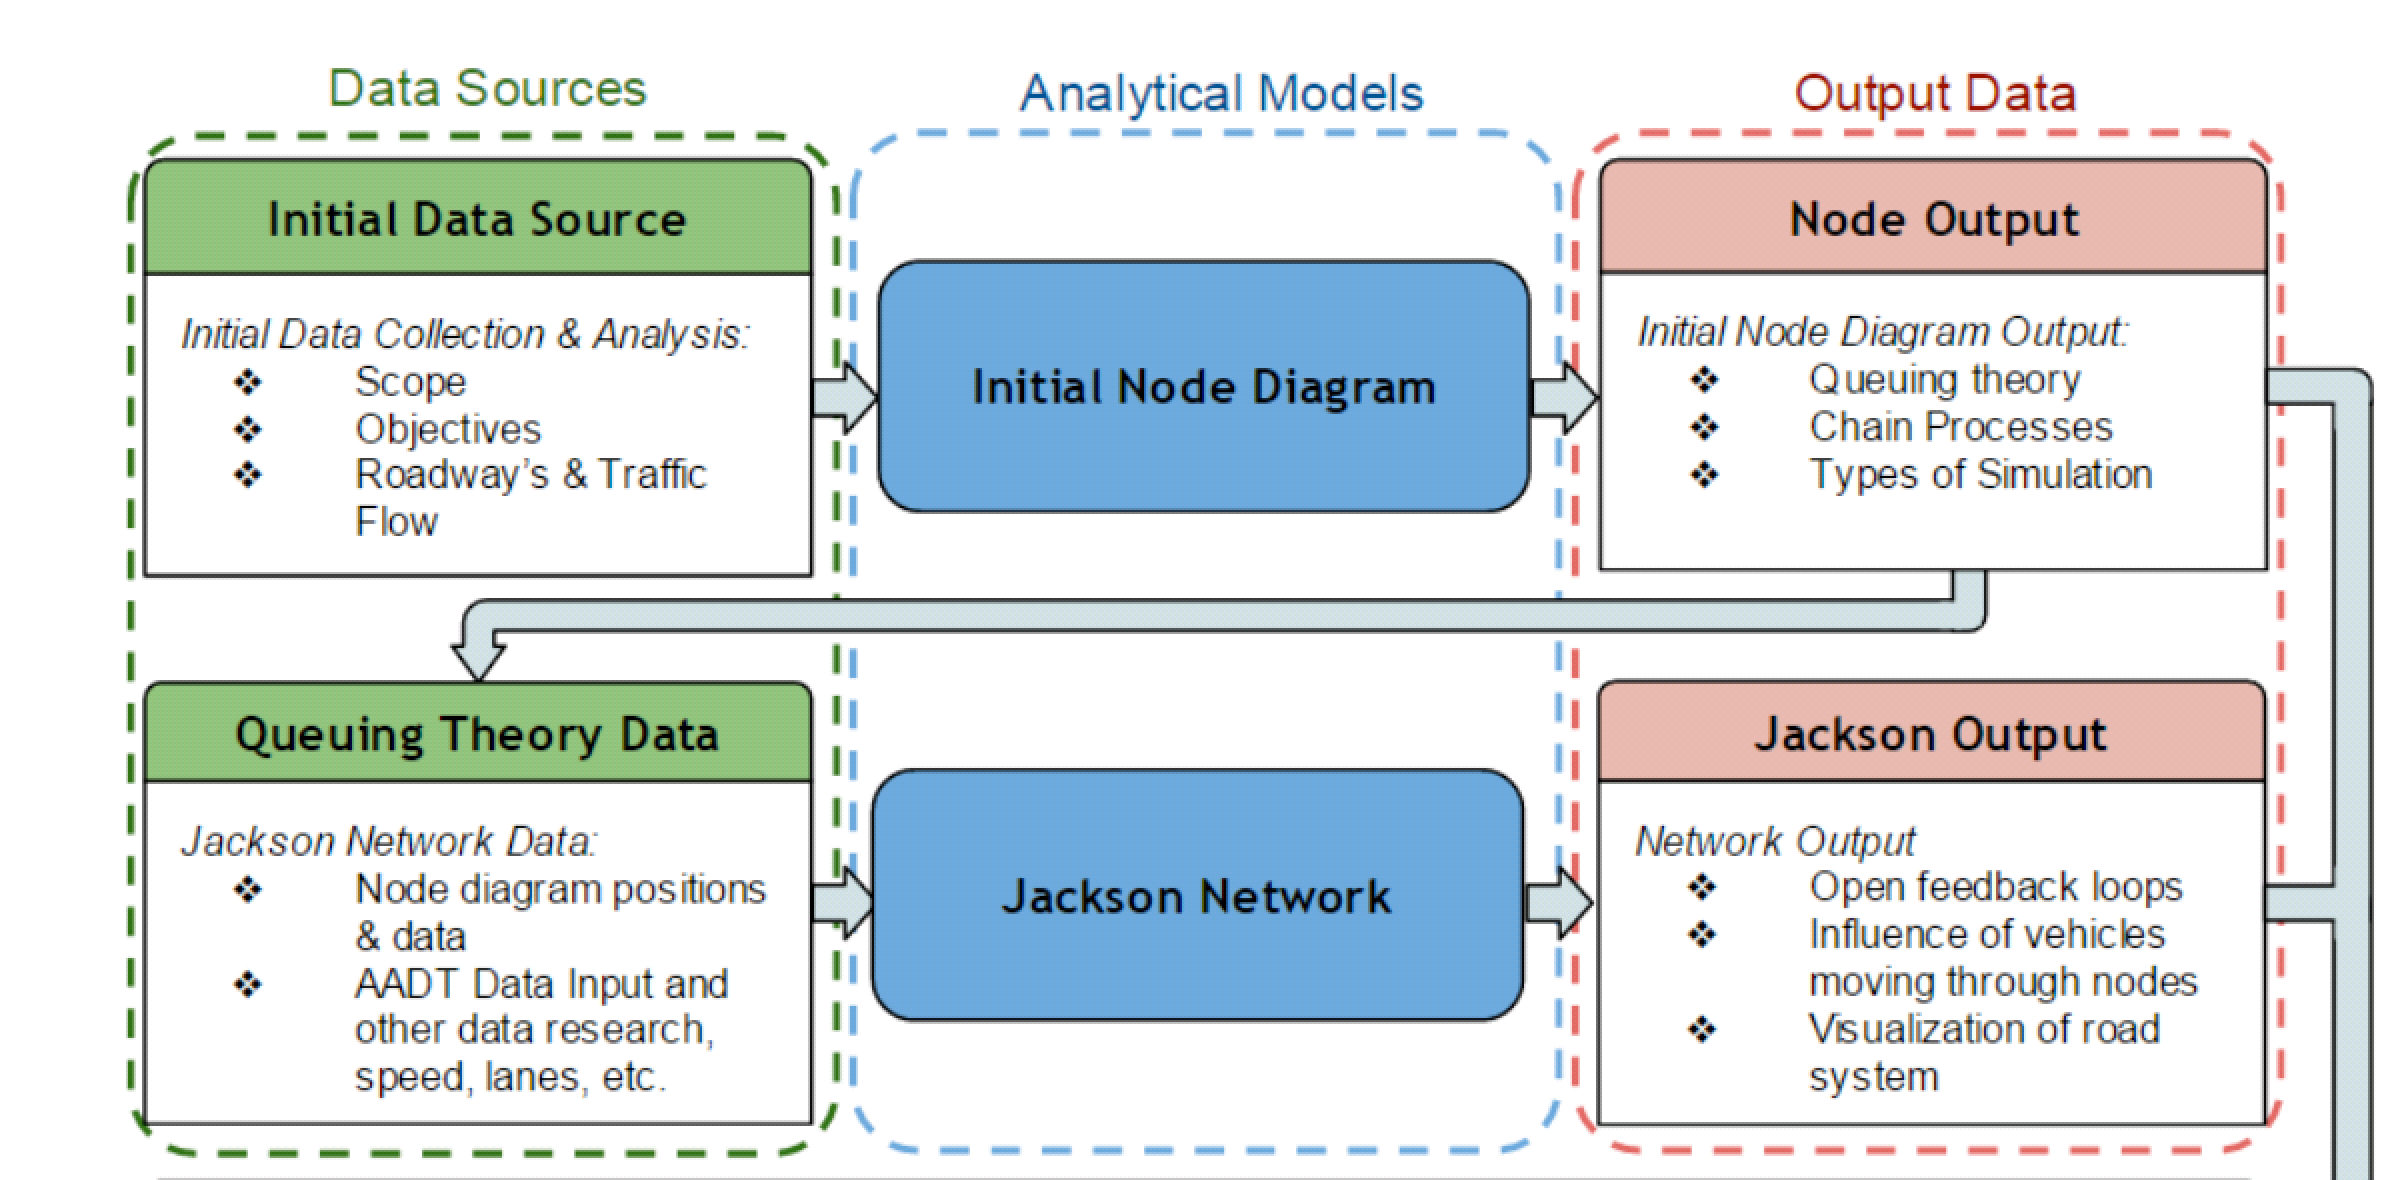
\includegraphics[width=3in]{picture/jackson_network}
						\caption{基于统计分析的关键路段识别模型}
						\label{jackson}
					\end{minipage}
			\end{figure}


	2017年,Yacine结合路段滑坡敏感性,给出了君士坦丁公路中路段的敏感性挖掘方法\parencite{Yacine2017Landslide},该方法结合路段的历史信息,通过解读航拍信息,遥感图像和实地调查,定义并研究了高速公路路段的滑坡性质。同时使用地理信息系统(GIS)为每个地理环境因素生成主题层图,从地质数据库中提取岩性单位和断层图的距离,结合数字高程模型(DEM)计算的斜坡坡度,坡度和距离,在GIS环境中对滑坡相关因素与滑坡事件之间的关系进行分析,获取易发生滑坡的路段。2014年,Ren等人基于节点的重要程度进行链接位置的优化,他们用节点的地理指标和集群特性来判定节点的重要程度,研究如何优化路段的连接方式和连接位置。这些方法从微观角度出发,通过研究节点和路段的特性来计算重要性,忽略了宏观交通流对整体网络的影响。

	2015年,Niu等人通过节点重要性评估方法研究关键节点\parencite{Niu2015Evaluation},他们提出了一种基于图论和网络理论评估公路网节点重要性的新方法,首先为每个具有GDP,里程,容量等权重的节点提出了一个效益函数,并计算出一个效益指标,表示每个节点的本地重要性;其次,为了描述整个网络的全球重要性,对节点之间的距离估计进行加权。通过地方和全球重要性的加权平均来计算每个节点的整体重要性。2011年,Song等人基于因子分析法,结合k-means算法对每个节点的重要程度进行进一步的划分\parencite{Song2011Node}。2011年,Wang等人基于节点的度、介数和交通量进行关键路段研究,同时结合C-means聚类方法进行进一步排序\parencite{Wang2011Signal}。2013年,他们又根据节点删除法来进行关键节点的识别\parencite{Wang2013Calculating},通过研究高速公路的级联失效性质,提出了基于节点失效、考虑连锁故障的交通网络节点重要性评估方法,它使用级联故障网络的拥塞状态来描述节点的重要性。2010年,Chen等人认为影响节点重要程度的因素有很多,而且它们的权值固定不变,基于这个思想,提出了一种基于Matlab聚类分析的解点重要性划分方法。

	2010年,Peeta等人提出了基于两层决策模型的关键路段挖掘方法\parencite{Peeta2010Pre},综合研究路段断裂后的连通性和路网通行效率,提出了一个度量高速公路路段重要性的模型。忽略路段之间的一阶联系,对离散函数进行求导,最终转化为背包问题进行线性时间复杂度的求解。该方法从宏观角度综合考虑了路段对整个高速公路系统的影响,但是该研究只针对桥梁,并且没有分析只考虑一阶路段影响的误差。

	现有的高速公路的关键路段研究较少,且大都是基于微观角度、基于统计学特性、基于路网结构求解,有各自的局限性。基于微观角度的研究方法虽然可以模拟真实情况下的路网状况,但是这类研究单纯的研究细节层面的高速公路网络规律,忽视了宏观层面的整体情况。基于统计学的研究方法虽然可以简单直观的根据历史先验经验,快速总结出规律,挖掘出路网的关键路段,但是这类基于经验的方法效果无法得到保证。基于网络拓扑结构虽然是研究各种复杂网络特性的经典方法,但是高速公路网络属于稀疏网络,网络复杂程度低,路网主要受到车流流量的影响。

\section{复杂网络关键路段挖掘相关研究}
	复杂网络中,关键节点的研究较多,关键路段的研究较少。因为传统的复杂网络(如社交网络)的边不具备实际的物理意义。近年来,复杂网络中节点重要性排序研究受到越来越广泛的关注。不同类型的网络中节点的重要性评价方法各有侧重,且应用领域极广,研究者们从不同的实际问题出发,设计出各种各样的方法。这些方法可以作为关键路段研究的参考。

	在交通研究中,可以对路网进行对偶拓扑,路段变成节点,节点变为边,关键路段挖掘转化为对路网中的关键节点挖掘。复杂网络关键节点研究中,主要用节点的空间分布、平均距离、连通性、聚类系数、度相关性等参数来度量节点的重要程度。用网络的抗毁性、传播、同步、控制等数据来测试网络的稳定性和完备性。基于复杂网络的关键节点挖掘算法研究较多,分类介绍。
				
	\subsection{基于节点临近}
		基于节点临近法是最简单直观的复杂网络关键路段挖掘方法,主要包含度中心性、半局部中心性、k-壳分解法等方法。

		度中心性的主要观点是:节点的重要性等价于该节点与其他节点的连接,使其具有的显著性。直观说来就是一个节点的邻居数目越多,他的影响力就越大\parencite{Phillip1972Factoring}。假设$v_i$是高速公路中的一个节点,$k_i$即为该节点的度,即为与该节点相连的节点的数目。在含权网络中,节点度定义为与节点相连的边的权重之和。度中心性刻画的是节点的直接影响力,一个节点的度中心性越大,证明该节点能够影响的邻居就越多,改节点就越重要。定义度中心性$L(i)$:

		$$L(i)=\frac{k_i}{n-1}$$

		式中的$k_i$代表节点的度,分母$n-1$代表整体路网的度之和。基于度中心性的关键路段挖掘方法具有简单、直观、计算复杂度低等特点。但是,他仅仅考虑了网络中节点的局部的信息,没有考虑对网络整体的拓扑结构、网络各个节点之间的深入联系。同时也缺乏对宏观层面的考虑。Chen等人提出了半局部中心性的想法\parencite{Chen2012Identifying},首先定义$N(v_i)$为节点$v_i$的两层邻居度,其值等于从$v_i$出发2跳(在路网中,直接相连的节点之间距离为1跳)内可到达的邻居的数目,$V_i^1$是距离节点$v_i$小于等于1跳的解点集合。然后定义$L(i)$:

		$$L(v_i)=\sum\limits_{v_i \in V_i^1} N(v_i)$$

		$v_i$的局部中心性定义为:
			$$F(v_i)=L(L(v_i))$$

		半局部中心性将度中心性由1跳扩展为4跳,不仅考虑了邻居节点的数量,还考虑了网络的聚类影响。在算法上达到了一定的提升。然而,研究表明节点在网络中的位置也是影响节点重要程度的重要因素。 在复杂网络中, 一个节点如果处于网络的核心位置,即使它的度中心性非常差,这个节点也往往具有很高影响力; 处在边缘的大度数节点影响力往往有限。Kitsak等人提出一种k-壳分解法\parencite{Kitsak2010Identification}。这个方法的思路是利用拓扑排序思路,将外围的节点层层剥去,节点存留时间越长,节点的重要性越大。k-壳分解法计算复杂度低, 当网络规模较大时,可以有效的分析网络的层级结构。然而,改方法不能应用于规则网络如树形图、星形图中。同时该方法的排序结果粒度太粗,节点的区分度不大。同时完全不考虑节点的度,显然不合理。Zeng 等人提出了在每一次迭代过程中,剥去最外层节点的同时,考虑节点剩余的邻居数$x_i$和节点已经移除的邻居数$y_i$的方法\parencite{Zeng2012Ranking}:定义节点$v_i$的混合度为$x_i+z*y_i$,不断计算新的混合度值,对网络分层。这种方法能够很好地区分树形图中不同节点的影响力,提高了节点传播能力的区分度。但是这个方法依然只局限于微观层面的结构特征,没有考虑宏观层面的影响。本文研究的是关键路段挖掘,关键路段的方法大都不能直接使用,但是可以给出一定的参考价值。
			

%05.02 查重。	
	\subsection{基于路径临近}
		在通信、交通、社交网络等网络结构中存在着一些很重要的边,这些边是连接几个区域的桥梁,它们在信息包和交通流的传递中担任重要的角色。此时,刻画节点重要性就需要考察网络中节点 对信息流的控制力, 这种控制力往往与网络中的路 径密切相关。 基于最短路径的排序方法假设网络中 的信息流只经过最短路径传输, 而真实的通信网络 中必须考虑负载平衡, 容错机制, 服务水平协议 (SLA)等\parencite{Dolev2010Routing}。 除了路径长度, 路径上的中间节点个数 对传播也有不可忽视的影响。 一对节点的中间节点 会增加这两个节点之间进行互动所需要的消耗。 第 一, 中间节点越多, 一对节点之间互动所需要的时间 就越长; 第二, 中间节点相当于在一对进行互动的节 点之间引入了“第三方”, 这会使传递的信息失真或 者延迟传递。 另一方面, 从提高网络的可靠性和抗毁 性角度看, 任意节点对之间的路径数目越多, 网络的 鲁棒性就越高。 此外类似于“桥节点”, 程学旗等人提 出了刻画网络边重要性的指标用来寻找“桥链路”, 相关讨论参见文献\parencite{Cheng2010Bridgeness}。

	在连通网络中, 定义$d_{ij}$为节点 $v_i$ 与 $v_j$ 之间的最 短路径长度, 也称最短距离, 一个节点 $v_i$的离心中心 性 (Eccentricity)为它与网络中所有节点的距离之中 的最大值\parencite{Hage1995Eccentricity}, 即:

\[ECC(i) = {\max _j}({d_{ij}})\]

				网络直径定义为网络 G 中所有节点的离心中心 性中的最大值, 网络半径定义为所有节点的离心中 心性值中的最小值。 显然, 网络的中心节点就是离心 中心性值等于网络半径的节点, 一个节点的离心中 心性与网络半径越接近就越中心。 要强调的是, 网络 直径在复杂网络研究中还有多种不同的定义, 例如 Albert 等人在研究万维网的时候定义网络直径为 网络中所有节点对的最短路径的平均值\parencite{Miro1997The}。 离心中心 性的缺点是极易受特殊值的影响, 如果一个节点与大部分节点的距离都很小, 只与极小部分节点的距 离很大,这个节点的离心中心性仍然会取其中的最大值。接近中心性则采取距离平均值的方式克服了 这一缺点。接近中心性(closeness centrality) 通过计算节
	点与网络中其他所有节点的距离的平均值来消除特 殊值的干扰。 一个节点与网络中其他节点的平均距 离越小, 该节点的接近中心性就越大。 接近中心性也可以理解为利用信息在网络中的平均传播时长来确
	定节点的重要性。 平均来说, 接近中心性最大的节点 对于信息的流动具有最佳的观察视野。 对于有 n 个节 点的连通网络, 可以计算任意一个节点$v_i$网络中 其他节点的平均最短距离:

\[{d_i} = \frac{1}{{n - 1}}\sum\limits_{j \ne i} {{d_{ij}}} \]

				$d_i$ 越小意味着节点 $v_i$ 更接近网络中的其他节点, 于是 把 $d_i$ 的倒数定义为节点 $v_i$ 的接近中心性, 即:

% MathType!MTEF!2!1!+-
% faaagCart1ev2aaaKnaaaaWenf2ys9wBH5garuavP1wzZbqedmvETj
% 2BSbqefm0B1jxALjharqqtubsr4rNCHbGeaGqiVu0Je9sqqrpepC0x
% bbL8FesqqrFfpeea0xe9Lq-Jc9vqaqpepm0xbba9pwe9Q8fs0-yqaq
% pepae9pg0FirpepeKkFr0xfr-xfr-xb9Gqpi0dc9adbaqaaeGaciGa
% aiaabeqaamaabaabaaGcbaGaam4qaiaadoeacaGGOaGaamyAaiaacM
% cacqGH9aqpdaWcaaqaaiaaigdaaeaacaWGKbWaaSbaaSqaaiaadMga
% aeqaaaaaaaa!35C4!
\[CC(i) = \frac{1}{{{d_i}}}\]

				上面定义的缺点是仅能用于连通的网络中, 文献\parencite{Latora2001Efficient} 在研究网络效率时对上式进行了改进, 使其能够用 于非连通网络中, 即:

				% MathType!MTEF!2!1!+-
% faaagCart1ev2aaaKnaaaaWenf2ys9wBH5garuavP1wzZbqedmvETj
% 2BSbqefm0B1jxALjharqqtubsr4rNCHbGeaGqiVu0Je9sqqrpepC0x
% bbL8FesqqrFfpeea0xe9Lq-Jc9vqaqpepm0xbba9pwe9Q8fs0-yqaq
% pepae9pg0FirpepeKkFr0xfr-xfr-xb9Gqpi0dc9adbaqaaeGaciGa
% aiaabeqaamaabaabaaGcbaGaamyraiaadAeacaWGgbGaaiikaiaadM
% gacaGGPaGaeyypa0ZaaabCaeaadaWcaaqaaiaaigdaaeaacaWGKbWa
% aSbaaSqaaiaadMgacaWGQbaabeaaaaaabaGaamOAaiabg2da9iaaig
% daaeaacaWGUbaaniabggHiLdaaaa!3D5D!
\[EFF(i) = \sum\limits_{j = 1}^n {\frac{1}{{{d_{ij}}}}} \]

				如果节点  $v_i$  和  $v_j$  之间没有路径可达则定义 $d_{ij}$  , 即$\frac{1}{d_{ij}}=0$。 接近中心性利用所有节点对之 间的相对距离确定节点的中心性, 在研究中应用非 常广泛, 但时间复杂度比较高。与接近中心性不同, Katz 中心性不仅考虑节点对 之间的最短路径, 还考虑它们之间的其他非最短路 径\parencite{Katz1953A}。Katz 中心性认为短路径比长路径更加重要, 它 通过一个与路径长度相关的因子对不同长度的路径 加权。 一个与$v_i$相距有 p 步长的节点, 对 $v_i$ 的中心性的贡献为$s^p$($s\in(0,1)$为一个固定参数)。 设$l_{ij}^{(p)}$为从 节点 $v_i$ 到 $v_j$ 经过长度为 p 的路径的数目。 显然 $A^2 =l_{ij}^{(2)}=(\sum\limits_k {a_{ik}a_{kj}})$, 其中元素$l_{ij}^{(2)}$即从节点 $v_i$ 到$v_j$经过的边数为 2 的路径的数目, 同理我们可以得到$A^3, A^4···A^p···, $将这些值赋予不同权重然后相加, 便可 以得到一个描述网络中任意节点对之间路径关系的 矩阵:
% MathType!MTEF!2!1!+-
% faaagCart1ev2aaaKnaaaaWenf2ys9wBH5garuavP1wzZbqedmvETj
% 2BSbqefm0B1jxALjharqqtubsr4rNCHbGeaGqiVu0Je9sqqrpepC0x
% bbL8FesqqrFfpeea0xe9Lq-Jc9vqaqpepm0xbba9pwe9Q8fs0-yqaq
% pepae9pg0FirpepeKkFr0xfr-xfr-xb9Gqpi0dc9adbaqaaeGaciGa
% aiaabeqaamaabaabaaGcbaGaam4saiabg2da9iaadohacaWGbbGaey
% 4kaSIaam4CamaaCaaaleqabaGaaGOmaaaakiaadgeadaahaaWcbeqa
% aiaaikdaaaGccqGHRaWkcaGGUaGaaiOlaiaac6cacqGHRaWkcaWGZb
% WaaWbaaSqabeaacaWGWbaaaOGaamyqamaaCaaaleqabaGaamiCaaaa
% kiabg2da9iaacIcacaWGjbGaeyOeI0Iaam4CaiaadgeacaGGPaWaaW
% baaSqabeaacqGHsislcaaIXaaaaOGaeyOeI0Iaamysaaaa!4795!
\[K = sA + {s^2}{A^2} + ... + {s^p}{A^p} = {(I - sA)^{ - 1}} - I\]

				其中,I为单位矩阵。K矩阵中第i行j列对应的元素$k_{ij}$ 实际上就是我们所熟知的节点 $v_i$ 和 $v_j$ 的 Katz 相似性\parencite{L2011Link}。 为保证 K 可写成公式(8)右侧的矩阵形式, 要求参数 s 小于邻接矩阵的最大特征值的倒数。 由此可定义一个节点 $v_j$ 的 Katz 中心性为矩阵 K 第 j 列元素的和:

				$$Katz(j)=\sum\limits_i {k_{ij}}$$

				Katz 中心性使用矩阵求逆的方法虽然比直接数 路径数目简单, 但时间复杂度依然比较高。 另一方面, 在考虑所有路径长度时, 如果节点 $v_i$ 与 $v_j$ 之间存在长 度为 p 的路径, 在使用 K 矩阵计算节点间长度为 p 的 奇数倍的路径时, 这条路径会被重复计算多次。 衰减 因子 s 的引入正好削弱了这些由于重复计算产生的 对中心性值的影响, 特别是当 s 很小时, 高阶路径的 贡献就非常小了, 使 Katz 指标的排序结果接近于局 部路径指标。 Katz 中心性主要用在规模不太大, 环路 比较少的网络中。 受到 Katz 中心性指标的启发, 我 们还可以应用其他刻画节点间相似性的指标\parencite{L2011Link}来定 义节点中心性。信息指标(information indices)\parencite{Stephenson1989Rethinking}通过路径中传播的信息量来衡量节点重要性。 该方法假定信息在一条边上传递的时候存在一定的噪音, 路径越长噪音就越大。 一条路径上的信息传输量等于该路径长度的倒数。 一对节点($v_i$, $v_j$)间能够传输的信息总量就等于它们之间所有路径传输的信息量之和, 记为 $q_{ij}$。值得注意的是, 如果我们把网络看成一个电阻网络,每条边的电阻记为 1, 则 1/$q_{ij}$ 相当于以 2 个节点 $v_i$ 和$v_j$ 为两端点的电阻值($q_{ij}$ 相当于电导)\parencite{Altmann1993Reinterpreting}, 于是我们可以通过计算矩阵$R=(r_{ij})=(D-A+F)^{-1}$获得$q_ij$, 其中D 是 n 阶对角矩阵, 对角线元素都是对应节点的度值, 非对角线元素为 0, F 是每个元素均为 1 的 n 阶方阵。 由此可得该网络中每一对节点($v_i$, $v_j$)间通过所有路径 能够传播的信息总量为

				$$q_{ij}=(r_{ii}+r_{jj}-2r_{ij})^{-1}$$

				最后, 用调和平均数的方法定义节点 $v_i$ 的中心性指标(有时也采用算术平均数)\parencite{Poulin2000Dynamical}:

				$$ INF(i)=[\frac{1}{n} \sum\limits_j {\frac{1}{q_{ij}}}] $$

				信息指标考虑了所有路径, 并可通过电阻网络 简化繁复的计算过程。 该方法可以很容易地扩展到 含权网络, 也适用于非连通的网络。
				可见, 无论是接近中心性、Katz 中心性还是信息 指标, 它们的思路是一致的。 如果用一个矩阵 M=($m_{ij}$) 来表示网络中所有节点之间的关系, M 的每一个元素 $m_{ij}$ 刻画了节点 $v_i$ 和 $v_j$ 之间的某种联系, 这个联系既 可以是它们之间的距离(如接近中心性), 也可以是某 种相似性, 于是一个节点 $v_i$ 的重要性可表示为Centrality(i)=$\sum\limits_j {m_{ij}}$。 由此可见, 只要我们能够给出一种刻画节点关系的方式, 就能够基于这个方法定 义一个节点的中心性。通常提到的介数中心性(betweenness centrality) 一般指最短路径介数中心性(shortest path BC), 它认 为网络中所有节点对的最短路径中(一般情况下一对 节点之间存在多条最短路径), 经过一个节点的最短 路径数越多, 这个节点就越重要。 介数中心性刻画了 节点对网络中沿最短路径传输的网络流的控制力。 节点$v_i$ 的介数定义为
% MathType!MTEF!2!1!+-
% faaagCart1ev2aaaKnaaaaWenf2ys9wBH5garuavP1wzZbqedmvETj
% 2BSbqefm0B1jxALjharqqtubsr4rNCHbGeaGqiVu0Je9sqqrpepC0x
% bbL8FesqqrFfpeea0xe9Lq-Jc9vqaqpepm0xbba9pwe9Q8fs0-yqaq
% pepae9pg0FirpepeKkFr0xfr-xfr-xb9Gqpi0dc9adbaqaaeGaciGa
% aiaabeqaamaabaabaaGcbaGaamOqaiaadoeacaGGOaGaamyAaiaacM
% cacqGH9aqpdaaeqbqaamaalaaabaGaam4zamaaDaaaleaacaWGZbGa
% amiDaaqaaiaadMgaaaaakeaacaWGNbWaaSbaaSqaaiaadohacaWG0b
% aabeaaaaaabaGaamyAaiabgcMi5kaadohacaGGSaGaamyAaiabgcMi
% 5kaadshacaGGSaGaam4CaiabgcMi5kaadshaaeqaniabggHiLdaaaa!489B!
\[BC(i) = \sum\limits_{i \ne s,i \ne t,s \ne t} {\frac{{g_{st}^i}}{{{g_{st}}}}} \]

				其中, $g_st$ 为从节点 $v_s$ 到 $v_t$ 的所有最短路径的数目, $g_{st}^i$为从节点 $v_s$到 $v_t$的 $g_{st}$ 条最短路径中经过 $v_i$ 的最短路 径的数目。 显然, 当一个节点不在任何一条最短路径 上时, 这个节点的介数中心性为 0, 比如星形图的外 围节点。 对于一个包含 n 个节点的连通网络, 节点度 的最大可能值为 n-1, 节点介数的最大可能值是星形 网络中心节点的介数值: 因为所有其他节点对之间 的最短路径是唯一的并且都会经过该中心节点, 所 以该节点的介数就是这些最短路径的数目, 于是得到一个归一化的介数:

				% MathType!MTEF!2!1!+-
% faaagCart1ev2aaaKnaaaaWenf2ys9wBH5garuavP1wzZbqedmvETj
% 2BSbqefm0B1jxALjharqqtubsr4rNCHbGeaGqiVu0Je9sqqrpepC0x
% bbL8FesqqrFfpeea0xe9Lq-Jc9vqaqpepm0xbba9pwe9Q8fs0-yqaq
% pepae9pg0FirpepeKkFr0xfr-xfr-xb9Gqpi0dc9adbaqaaeGaciGa
% aiaabeqaamaabaabaaGcbaGaamOqaiaadoeadaahaaWcbeqaaiaacE
% caaaGccaGGOaGaamyAaiaacMcacqGH9aqpdaWcaaqaaiaaikdaaeaa
% caGGOaGaamOBaiabgkHiTiaaigdacaGGPaGaaiikaiaad6gacqGHsi
% slcaaIYaGaaiykaaaadaaeabqaamaalaaabaGaam4zamaaDaaaleaa
% caWGZbGaamiDaaqaaiaadMgaaaaakeaacaWGNbWaaSbaaSqaaiaado
% hacaWG0baabeaaaaaabeqab0GaeyyeIuoaaaa!45B0!
\[BC^{'}(i) = \frac{2}{{(n - 1)(n - 2)}}\sum {\frac{{g_{st}^i}}{{{g_{st}}}}} \]

				介数中心性可用于设计网络的通信协议、优化网 络部署、检测网络瓶颈等。Goh 等人提出的负载中心性(traffic load centrality)采用类似网络中信息包传递的机制\parencite{Goh2001Universal}: 每一 对节点之间沿着最短路径传输一个单位的网络流, 如果最短路径不止一条, 则在几条最短路径的分叉 处将网络流平均分配到这些最短路径上。 忽略时延, 网络中所有节点对之间都互不干扰地传输一个单位 的信息流时, 一个节点上传输过的网络流的数量称 为该节点的负载。 一个节点的负载越大, 该节点就越 重要。 介数中心性的计算时间复杂度较高, 使其在实 际应用中受到限制, 相关讨论可参见文献\parencite{Ulrik2001A,zt2006Notes}。介数中心性仅考虑网络流通过最短路径传输。 Yan 等人\parencite{Yan2006Efficient}的研究指出, 如果选择最短路径来运输 网络流, 很多情况下反而会延长出行时间、降低出行 效率。 把一对节点之间的每条路径看作一条单独的 管道, 一条管道能够传输一个单位的网络流, 从源节 点 $v_s$ 到目标节点 $v_t$ 的最大流量是指 $v_s$ 与 $v_t$ 之间所有 管道可同时运输的网络流的总和(实际上, 这种假设 没有实际意义, 多条路径往往有重合的部分, 重合部 分的流量就会超过假设的情况)。 基于这样的假设, 流介数中心性(flow betweenness centrality)\parencite{}认为网 络中所有不重复的路径中, 经过一个节点的路径的 比例越大, 这个节点就越重要。 由此得到节点 $v_i$ 的流 介数中心性为

			\[FBC^{'}(i) = \sum\limits_{s<t} {\frac{{g_{st}^i}}{{{g_{st}}}}} \]


				介数中心性和流介数中心性考虑的是两个极端, 前 者只考虑最短路径, 后者考虑所有路径并认为每条 路径作用相同, 接下来介绍两种介于两者之间的介 数中心性算法。首先介绍随机游走介数中心性:从源节点 $v_s$ 到目标节点 $v_t$ 的随机游走的过程中 当i=s或者t的时候,$I_{st}^s=I_{st}^t=1$。该方法计算复杂度较高。路由介数中心性:计算机网络中, 每个路由器都有一个包含很多行记录的路由表, 每行记录存储着要到达的目标地址及下一跳地址。 显然, 每个路由器只记录了局部的网络结构信息。 对网络中的每一对节点($v_s$, $v_t$), 将分布在各个路由器中的信息聚合, 可形成一个关于这一对节点的有向无环图 R(s, t)。 定义 p(s, u, v, t)为有向无环图 R(s, t)中节点 $v_u$ 转发给节点 $v_v$ 一个从源节点$v_s$ 到目标节点 $v_t$ 的信息包的概率。 如果 p(s, u, v, t)>0,则在 R(s, t)中存在一条从 $v_u$ 指向 $v_v$ 的有向边。 用$k_{s,t}^{(u)}$表示信息包从 $v_s$ 到 $v_t$的传递过程中, 经过节点的 $v_u$概率, 显然$k_{s,t}^{(s)}=k_{s,t}^{(t)}=1$, 用 $Pred_{s,t}^{(v)}$表示 。 那么有向无环图 R(s, t)中 经过任意一个节点 $v_v$ 的概率可由下式得出:

				% MathType!MTEF!2!1!+-
% faaagCart1ev2aaaKnaaaaWenf2ys9wBH5garuavP1wzZbqedmvETj
% 2BSbqefm0B1jxALjharqqtubsr4rNCHbGeaGqiVu0Je9sqqrpepC0x
% bbL8FesqqrFfpeea0xe9Lq-Jc9vqaqpepm0xbba9pwe9Q8fs0-yqaq
% pepae9pg0FirpepeKkFr0xfr-xfr-xb9Gqpi0dc9adbaqaaeGaciGa
% aiaabeqaamaabaabaaGcbaGaam4samaaBaaaleaacaWGZbGaaiilai
% aadshaaeqaaOGaaiikaiaadAhacaGGPaGaeyypa0ZaaabuaeaacaWG
% lbWaaSbaaSqaaiaadohacaGGSaGaamiDaaqabaGccaGGOaGaamyDai
% aacMcacaWGWbGaaiikaiaadohacaGGSaGaamyDaiaacYcacaWG2bGa
% aiilaiaadshacaGGPaaaleaacaWG1bGaeyicI4Saciiuaiaackhaca
% WGLbGaamizamaaBaaameaacaWGZbGaaiilaiaadshaaeqaaSGaaiik
% aiaadAhacaGGPaaabeqdcqGHris5aaaa!50C5!
\[{K_{s,t}}(v) = \sum\limits_{u \in \Pr e{d_{s,t}}(v)} {{K_{s,t}}(u)p(s,u,v,t)} \]

我们考虑经过节点的路径为一个封闭环的时候, 就可以定义子图中心性(subgraph centrality)\parencite{Estrada2005Subgraph}。该方法从全局的视野考察了网络中所有可达的邻居对节点中心性的增强作用, 并且认为增强作用会随距离的增加而衰减。 与图论中的概念有所不同, 这里一个子图特指从一个节点开始到这个节点结束的一条闭环回路。 一个节点 $v_i$ 的子图数目就是以该节点为首尾的闭环回路的个数。 子图中心性认为闭环回路的路径长度越小, 回路信息交流越便利, 节点之间的联系越紧密, 对节点的中心性贡献越大, 其定义为

			% MathType!MTEF!2!1!+-
% faaagCart1ev2aaaKnaaaaWenf2ys9wBH5garuavP1wzZbqedmvETj
% 2BSbqefm0B1jxALjharqqtubsr4rNCHbGeaGqiVu0Je9sqqrpepC0x
% bbL8FesqqrFfpeea0xe9Lq-Jc9vqaqpepm0xbba9pwe9Q8fs0-yqaq
% pepae9pg0FirpepeKkFr0xfr-xfr-xb9Gqpi0dc9adbaqaaeGaciGa
% aiaabeqaamaabaabaaGcbaGaam4uaiaadoeacaGGOaGaamyAaiaacM
% cacqGH9aqpdaaeWbqaamaalaaabaGaamyyamaaDaaaleaacaWGPbGa
% amyAaaqaaiaadshaaaaakeaacaWG0bGaaiyiaaaaaSqaaiaadMgacq
% GH9aqpcaaIXaaabaGaeyOhIukaniabggHiLdaaaa!3F08!
\[SC(i) = \sum\limits_{i = 1}^\infty  {\frac{{a_{ii}^t}}{{t!}}} \]

				其中$a_{ii}^t$为网络的邻接矩阵A的t次幂的第i个对角线元素。t=1时, $a_{ii}^1=0$;t=2时, $a_{ii}^2$为节点v 的度值, 即 $a_{ii}^2=k$ , 此时, 子图中心性就等价于度中心性; $t>2$ 时, $a_{ii}^t=k$ 表示从点$v_i$开始,经过t条边又回到$v_i$的路径 的数目。 子图中心性赋予较短的回路较高的权重, 使 得节点的度在其中发挥较大作用的同时, 还考虑了 高阶回路。 在实际应用时, 根据具体计算需求, t 可 以取到任意值截断。 子图中心性用邻接矩阵特征值 和特征向量可表示为

				% MathType!MTEF!2!1!+-
% faaagCart1ev2aaaKnaaaaWenf2ys9wBH5garuavP1wzZbqedmvETj
% 2BSbqefm0B1jxALjharqqtubsr4rNCHbGeaGqiVu0Je9sqqrpepC0x
% bbL8FesqqrFfpeea0xe9Lq-Jc9vqaqpepm0xbba9pwe9Q8fs0-yqaq
% pepae9pg0FirpepeKkFr0xfr-xfr-xb9Gqpi0dc9adbaqaaeGaciGa
% aiaabeqaamaabaabaaGcbaGaam4uaiaadoeacaGGOaGaamyAaiaacM
% cacqGH9aqpdaaeWbqaamaalaaabaGaamyyamaaDaaaleaacaWGPbGa
% amyAaaqaaiaadshaaaaakeaacaWG0bGaaiyiaaaaaSqaaiaadMgacq
% GH9aqpcaaIXaaabaGaeyOhIukaniabggHiLdGccqGH9aqpdaaeWbqa
% aiaacIcacaWGlbWaa0baaSqaaiaadMgaaeaacaWGQbaaaOGaaiykam
% aaCaaaleqabaGaaGOmaaaaaeaacaWGQbGaeyypa0JaaGymaaqaaiaa
% d6eaa0GaeyyeIuoakiaadwgadaahaaWcbeqaaiaadYgadaWgaaadba
% GaamOAaaqabaaaaaaa!4E26!
\[SC(i) = \sum\limits_{i = 1}^\infty  {\frac{{a_{ii}^t}}{{t!}}}  = \sum\limits_{j = 1}^N {{{(K_i^j)}^2}} {e^{{l_j}}}\]

				其中,$l_j$为邻接矩阵A的特征值,$K_j$是$l_i$所对应的特征向量,$K_i^j$表示特征向量的第 i 个元素。 有些情况下, 度中心性, 接近中心性以及介数 中心性都不能区分网络中某些节点谁更重要时, 可 用子图中心性来对这些节点进行更加细致地区分\parencite{Estrada2005Subgraph}。 另外, 子图中心性的方法还能够应用于网络中模体 的检测\parencite{Estrada2005Subgraph}。



	\subsection{基于特征向量的排序方法}
	前面介绍的方法都是从邻居的数量上考虑对节 点重要性的影响, 基于特征向量的方法不仅考虑节 点邻居数量还考虑了其质量对节点重要性的影响。 下面将详细介绍 7 种方法。 其中前两种方法, 即特征 向量中心性和累计提名方法一般用在无向网络中, 后者收敛更快。 后面五种方法可看成特征向量中心性 在有向网络中的应用。 PageRank 算法和 LeaderRank 算 法通过模拟用户上网浏览网页的过程, 使节点的分 值沿着访问路径增加, 用于识别网页重要性。 实验结 果显示, LeaderRank 表现好于 PageRank 算法。 HITs 算法、自动信息汇集算法, SALSA 算法中考虑节点的 双重角色: 权威性和枢纽性, 并认为两者相互影响。 本类方法在理论和商业上都受到了极大的关注, 很 有借鉴意义。

	特征向量中心性(eigenvector centrality)\parencite{Phillip1972Factoring}认为一 个节点的重要性既取决于其邻居节点的数量(即该节 点的度), 也取决于每个邻居节点的重要性。 记 $x_i$ 为 节点 v 的重要性度量值, 则:

				$$EC(i)=x_i=c\sum\limits_{j=1}^n {a_{ij}x_j}$$

				特征向量中心性更 加强调节点所处的周围环境(节点的邻居数量和质 量), 它的本质是一个节点的分值是它的邻居的分值 之和, 节点可以通过连接很多其他重要的节点来提 升自身的重要性, 分值比较高的节点要么和大量一 般节点相连, 要么和少量其他高分值的节点相连。 从 传播的角度看, 特征向量中心性适合于描述节点的 长期影响力, 如在疾病传播、谣言扩散中, 一个节点 的 EC 分值较大说明该节点距离传染源更近的可能性 越大, 是需要防范的关键路段。
				特征向量法完全用与某节点相连接的其他节点 的信息来评价该节点的重要性。 Bonacich 等人\parencite{Bonacich2001Eigenvector}认为 节点的重要性还可能受到不依赖于节点连接信息的 一些来自外部的信息的影响。 例如在微博上有人喜 爱转发其他人发布的信息(依赖于网络连接的内部信 息), 有的人却比较热衷于发布原创信息或从其他网 站转发一些信息(不依赖于网络连接的外部信息)。 由 此 Bonacich 等人提出阿尔法中心性(Alpha-centrality), 即 $x=\alpha Ax+e$, 其中$\alpha$ 为刻画来自网络内部连接影响的 内因参数, e 为刻画那些不受网络连接影响的外因参 数。 不失一般性,e可以设置为一个所有元素都等于1 的向量, 此时阿尔法中心性与 Katz 中心性一致。
				当网络中有一些度特别大的节点的时候, 特征 向量中心性会出现分数局于化现象(Localiztion), 即 大多数分值都集中在大度节点上, 使得其他节点的 分值区分度很低。 为了避免这一现象, Martin 等人\parencite{Martin2015Localization} 对特征向量中心性进行改进, 提出在计算节点$v_i$的分 值时, 求和中其邻居的分值不再考虑节点$v_i$的影响。特征向量中心性中, 一个节点的打分值完全由邻居决定, 收敛过程缓慢。 此外, 当不存在一个正的自然数 t, 使得转移矩阵的 t 次幂所有元素都是正的时, 节点打分值会出现周期性循环, 不能收敛。 为了使打分值能够收敛并且快速收敛, 累计提名(cumulative nomination) \parencite{Wei2013Identifying}方法在每次迭代过程中,同时考虑邻居节点和自身的打分值。 设 $p_i^t$ 为节点 $v_i$在时刻 t 时得到的提名次数, 假设 t=0 时每个节点都获得 1 次提名(即 $p_i^0 =1$ ), 每个时间步每个节点从所 i有相邻的节点处获得新增的提名, 新增的提名数为 邻居节点已有的提名数的总和。 于是定义节点在 t+1 时刻的累积提名为

			% MathType!MTEF!2!1!+-
% faaagCart1ev2aaaKnaaaaWenf2ys9wBH5garuavP1wzZbqedmvETj
% 2BSbqefm0B1jxALjharqqtubsr4rNCHbGeaGqiVu0Je9sqqrpepC0x
% bbL8FesqqrFfpeea0xe9Lq-Jc9vqaqpepm0xbba9pwe9Q8fs0-yqaq
% pepae9pg0FirpepeKkFr0xfr-xfr-xb9Gqpi0dc9adbaqaaeGaciGa
% aiaabeqaamaabaabaaGcbaGaamiCamaaDaaaleaacaWGPbaabaGaam
% iDaiabgUcaRiaaigdaaaGccqGH9aqpcaWGWbWaa0baaSqaaiaadMga
% aeaacaWG0baaaOGaey4kaSYaaabuaeaacaWGHbWaaSbaaSqaaiaadM
% gacaWGQbaabeaakiaadchadaqhaaWcbaGaamOAaaqaaiaadshaaaaa
% baGaamOAaaqab0GaeyyeIuoaaaa!40CE!
\[p_i^{t + 1} = p_i^t + \sum\limits_j {{a_{ij}}p_j^t} \]

				如果所有节点归一化后的提名次数不再变化, 则停 止迭代。 稳态时每个节点的提名次数占所有节点的 提名次数的比例就是其重要性权值。 特征向量中心 性算法在每次迭代的时候, 一个节点 $v_i$ 的中心性值 完全等于邻居的中心性值之和, 而累计提名算法则 保留了节点 $v_i$ 上一步的中心性值, 实验结果显示累 积提名相比原始的特征向量中心性收敛速度更快。 累积提名和 Alpha 中心性在数学形式上非常相似, 但 Alpha 中心性中的 e 是固定值, 即每次迭代的时候不 变, 而累积提名中添加的是上一时间步的打分值, 这 个打分值会随着每步更新变化。

				特征向量中心性及其变体应用广泛, 例如网页 排序领域中最著名的 PageRank 算法, 是谷歌搜索 引擎的核心算法。 传统的根据关键字密度判定网页 重要程度的方法容易受到“恶意关键字”行为的诱导, 使搜索结果可信度低。 PageRank 算法基于网页的链 接结构给网页排序, 它认为万维网中一个页面的重 要性取决于指向它的其他页面的数量和质量, 如果 一个页面被很多高质量页面指向, 则这个页面的质 量也高。 初始时刻, 赋予每个节点(网页)相同的 PR 值, 然后进行迭代, 每一步把每个节点当前的 PR 值 平分给它所指向的所有节点。 每个节点的新 PR 值为 它所获得的 PR 值之和, 于是得到节点 $v_i$ 在 t 时刻的 PR 值为

			% MathType!MTEF!2!1!+-
% faaagCart1ev2aaaKnaaaaWenf2ys9wBH5garuavP1wzZbqedmvETj
% 2BSbqefm0B1jxALjharqqtubsr4rNCHbGeaGqiVu0Je9sqqrpepC0x
% bbL8FesqqrFfpeea0xe9Lq-Jc9vqaqpepm0xbba9pwe9Q8fs0-yqaq
% pepae9pg0FirpepeKkFr0xfr-xfr-xb9Gqpi0dc9adbaqaaeGaciGa
% aiaabeqaamaabaabaaGcbaGaamiuaiaadkfadaWgaaWcbaGaamyAaa
% qabaGccaGGOaGaamiDaiaacMcacqGH9aqpdaaeWbqaaiaadggadaWg
% aaWcbaGaamOAaiaadMgaaeqaaOWaaSaaaeaacaWGqbGaamOuamaaBa
% aaleaacaWGQbaabeaakiaacIcacaWG0bGaeyOeI0IaaGymaiaacMca
% aeaacaWGRbWaa0baaSqaaiaadQgaaeaacaWGVbGaamyDaiaadshaaa
% aaaaqaaiaadQgacqGH9aqpcaaIXaaabaGaamOBaaqdcqGHris5aaaa
% !48E2!
\[P{R_i}(t) = \sum\limits_{j = 1}^n {{a_{ji}}\frac{{P{R_j}(t - 1)}}{{k_j^{out}}}} \]

				迭代到每个PR值都达到稳定时为止。 公式的缺陷在于 PR 值一 旦到达某个出度为零的节点(称为悬挂节点 Dangling node), 就会永远停留在该节点处而无法传递出来, 从而不断吸收 PR 值。 为解决这一问题, PageRank 算法在上述过程基础上引入一个随机跳转概率 c。 每 一步, 不管一个节点是否为悬挂节点, 其 PR 值都将以 c 的概率均分给网络中所有节点, 以 1-c 的概率均 分给它指向的节点。 该过程实际上是考虑到了现实 中网络用户除了通过超链接访问页面之外, 还可以 通过直接输入网址的形式对网页进行访问的行为, 从而保证了即使是没有任何入度的网页也有机会被 访问到。 其实质是将有向网络变成强连通的, 使邻接 矩阵成为不可约矩阵, 保证了特征值 1 的存在。 由此 可得含参数 c 的 PageRank 算法:

% MathType!MTEF!2!1!+-
% faaagCart1ev2aaaKnaaaaWenf2ys9wBH5garuavP1wzZbqedmvETj
% 2BSbqefm0B1jxALjharqqtubsr4rNCHbGeaGqiVu0Je9sqqrpepC0x
% bbL8FesqqrFfpeea0xe9Lq-Jc9vqaqpepm0xbba9pwe9Q8fs0-yqaq
% pepae9pg0FirpepeKkFr0xfr-xfr-xb9Gqpi0dc9adbaqaaeGaciGa
% aiaabeqaamaabaabaaGcbaGaamiuaiaadkfadaWgaaWcbaGaamyAaa
% qabaGccaGGOaGaamiDaiaacMcacqGH9aqpcaGGOaGaaGymaiabgkHi
% TiaadogacaGGPaWaaabCaeaacaWGHbWaaSbaaSqaaiaadQgacaWGPb
% aabeaakmaalaaabaGaamiuaiaadkfadaWgaaWcbaGaamOAaaqabaGc
% caGGOaGaamiDaiabgkHiTiaaigdacaGGPaaabaGaam4AamaaDaaale
% aacaWGQbaabaGaam4BaiaadwhacaWG0baaaaaaaeaacaWGQbGaeyyp
% a0JaaGymaaqaaiaad6gaa0GaeyyeIuoakiabgUcaRmaalaaabaGaam
% 4yaaqaaiaad6gaaaaaaa!4FA2!
\[P{R_i}(t) = (1 - c)\sum\limits_{j = 1}^n {{a_{ji}}\frac{{P{R_j}(t - 1)}}{{k_j^{out}}}}  + \frac{c}{n}\]

				参数 c 的取值要视具体的情况而定。 c 取值越大收敛越快。 c 取值越大算法的有 效性越低, c=1 时所有节点都有相同的 PR 值。 针对万 维网的网页排序, 以前的研究显示, c=0.15 是一个比 较好的参数。 PageRank 算法作为谷歌搜索引擎的核 心算法, 它在商业应用上的极大成功激发了人们深 入研究 PageRank 的热忱, 研究者们提出了一系列基 于 PageRank 的改进算法。 例如 Kim 和 Lee\parencite{Kim2002An}为了避 免悬挂节点囤积 PR 值的问题, 将每一步到达悬挂节 点的 PR 值平均分给网络中的 n 个节点, 即将概率转 移矩阵中悬挂节点所在的列的 n 个元素修改为 1/n; PageRank 中从一个网页上的链接中挑选下一个访问 目标时是等概率的, Zhang 等人\parencite{Zhang2007N}认为这 n 个目标网 页出度越大的越有可能被点击, 并提出 N-step PageRank 算法用以描述这一思想。 2012 年 Brin 和 Page\parencite{Sergey1998The}以相同的题目重新出版了当年提出 PageRank 算法的博士学位论文, 在文中他们对这十几年的网 页排序算法进行了回顾, 并就如何用 PageRank 实现 大规模搜索进行了深入讨论。 另外, 作为有向网络节 点排序最经典的算法, PageRank 及其改进算法广泛 应用于其他领域, 如对期刊的排序\parencite{Jacso2012Grim}、对社交网络上 用户的排序\parencite{Weng2010TwitterRank}、对风投公司(VC)的排序\parencite{Bhat2012InvestorRank}、对科学论 文的排序\parencite{Petersen2010Methods}以及科学家影响力的排序\parencite{Ding2009PageRank}等。


	\subsection{基于节点移除和收缩的排序方法}
	节点(集)的移除和收缩方法与系统科学中确定一个系统的核心的思路暗合 , 其最显著的特点是在重要节点排序的过程中, 网络的结构会处于动态 变化之中, 节点的重要性往往体现在该节点被移除 之后对网络的破坏性。 从衡量网络的健壮性角度看, 一些节点一旦失效或移除, 网络就有可能陷入瘫痪 或者分化为若干个不连通的子网。 实际生活中的很 多基础设施网络, 如输电网、交通运输网、自来水- 天然气供应网络等, 都存在“一点故障, 全网瘫痪”的 风险。 为了预防风险, 研究人员提出了很多方法来研 究节点收缩或者移除之后网络的结构与功能的变化, 从而为新系统的设计与建造提供依据。 比较典型的 是系统的“核与核度”理论。 许进等人在定义规则 网络图的核概念基础上, 提出了核度的测量方法, 研 究了网络核度与节点数、边数的关系, 并根据它们之 间的关系设计了规则网络构造定理; 李鹏翔等人认为直接的联系往往是间接联系的必经之路, 在评 估节点重要性的过程中更加重要, 用节点集被删除 后形成的所有不直接相连的节点对之间的最短距离 的倒数之和来反映节点删除对网络连通的破坏程度; 陈勇等人分析了通信网络, 考察去掉节点(集)及其 相关边后所得到的图的生成树的数目, 数目越小, 表 明该节点(集)越重要; 谭跃进等人用收缩节点方法 替代删除节点法, 综合考虑了节点的度以及经过该 节点的最短路径的数目, 将节点收缩后网络的聚集 度作为节点重要性评估的标准。 系统科学的方法给 我们提供了新的视角, 但由于计算复杂度较高, 目前 这类方法还仅限于小规模的网络实验。 此外, Restrepo 等人\parencite{Restrepo2006Characterizing}提出通过考察网络最大特征值在移除节点后的变化来衡量节点重要性的方法, 该方法还可以应 用于刻画网络连边的重要性。


	破坏性反映重要性。 节点删除的最短距离法\parencite{lpx2004wl} 认为一个节点移除后的破坏性与所引起的距离变化 有关: 移除一个节点(集)会引起网络分化, 并形成若 干个连通分支, 网络中节点对之间较短距离的变化 越大, 被移除的节点就越重要。 该算法区别对待不同 长度的路径, 认为“相对直接的、近距离的联系所造 成的破坏性大于相对间接的、远距离的联系所造成的 破坏性”\parencite{lpx2004wl}。 具体地, 在连通图中一个节点被删除之 后, 对网络的整体状况的影响体现在两个方面: 直接 损失和间接损失。
				直接损失是指被删除的节点与其他剩余的节点之间不再存在通路, 如果连通网络中共有 n 个节点,删除一个节点后产生的不连通节点对的数目为 n-1。如果删除的是节点集, 直接损失还应该包括删除的节点集内节点之间的不再连接的损失。 间接损失是指删除一个节点造成剩余节点之间不连通而引发的损失: 用 $N_k$ (k=1, 2, ···, s)表示一个节点 $v_i$ 被删除后,网络分化成的 s 个连通子图中第 k 个连通子图的节点数, 则该节点被删除后所形成的不再连通的节点对的数目为$\sum\limits_{t = 1}^s {\sum\limits_{r = t + 1}^s {{N_t}{N_r}} } $ , 记由于删除节点 $v_i$ 造成的不再相连的节点对表示为集合 E (包括直接损失和 间接损失两部分), 那么节点 $v_i$ 的重要性等于集合 E 中节点对之间的最短距离的倒数之和, 即:

$$DSP(i)=\sum\limits_{(j,k)\in E} {\frac{1}{d_{jk}}}$$
				

				$d_{jk}$为删除节点$v_i$之前$v_j$与$v_k$间的最短距离。 注意, 当 j或k=i的时候, 相当于直接损失; 当 $j\ne k\ne i$的时候, 相当于间接损失。 节点删除的最短距离法在衡量一 些节点集的重要性方面优势比较突出。 在实际的大 规模网络中, 仅删除一个节点时网络的拓扑图一般 不会分化为几个连通子图, 网络的间接损失为 0, 节 点删除的最短距离法效果并不明显。 而如果同时删 除多个节点, 则很容易使网络不再连通, 这时该方法 的优越性就显现出来了。

			在通信网络中, 节点删除后网络中节点对之间最短距离会发生变化, 但一般对网络时延影响不大,用最短距离法不一定准确。 这时可通过考察节点删 除后网络拓扑图的生成树个数来衡量节点的重要性。 在图论中, 一个图的树是该图的一个连通的无环子 图, 一个图的生成树定义为拥有该图的所有顶点的 树。 节点删除的生成树法\parencite{cy2004tx}认为一个节点删除后对 应的网络的生成树的数目越少, 该节点越重要。 给定 一个无向连通图, 其邻接矩阵为 A, 网络拉普拉斯矩 阵 L=D–A(将矩阵 A 主对角线上的元素 $a_{ii}$ 替换为节点 $v_i$ 的度值, 非对角线上的元素值全部乘以-1)。 那么, 这个连通无向图的生成树个数 $t_0$ 为矩阵 L 的任意一 个元素$l_pq$的余子式$M_pq$的行列式, 即: $t_0 = \|M_{pq}\|$ 。 删除任意一个节点$v_i$, 网络的邻接矩阵变为$A_{-i}$, 然后用 上面的方法计算网络的生成树个数为 $t_{-i}$。 由此可定 义节点$v_i$ 的中心性指标为

				$$DST(i)=1-\frac{t_{-i}}{t_0}$$

				在节点的移除对网络的连通性影响不大的网络 中, 节点删除的生成树法优于最短距离法。 但节点删 除的生成树法有一些缺点, 例如, 只能用在连通网络 中。 若一个节点删除后网络变得不再连通, 这些节点 的重要性就难以判断了, 这时可采用节点收缩法评 估节点的重要性。

				节点收缩就是将一个节点和它的邻节点收缩成 一个新节点\parencite{tyj2006fz}。 如果 $v_i$ 是一个很重要的核心节点, 将 它收缩后整个网络将能更好地凝聚在一起。 最典型 的就是星形网络的核心节点收缩后, 整个网络就会 凝聚为一个大节点。 从社会学的角度讲, 社交网络中 人员之间联系越方便(平均最短路径长度 d 越小), 人 数越少(节点数 n 越小), 网络的凝聚程度就越高。 因 此定义网络的凝聚度为

				$$A[G]=\frac {1}{nd}=\frac{1}{n \frac{\sum\limits_{i\ne j} {d_{ij}}} {n(n-1)}} = \frac{n-1}{\sum\limits_{i\ne j} {d_{ij}}}$$

				可见, 节点收缩法中节点的重要程度由节点的邻居数量和节点在网络路径中的位置共同决定。 由于每 次收缩一个节点, 都要计算一次网络的平均路径长度, 时间复杂度比较高, 不适于计算大规模网络。

				为了研究网络的抗毁性, Dangalchev\parencite{Dangalchev2006Residual}提出了残 余接近中心性(residual closeness centrality), 用来衡 量节点的移除对网络带来的影响。 残余接近中心性 认为若一个节点的删除使得网络变得更加脆弱, 该 节点就越重要。 文献\parencite{Dangalchev2006Residual}对接近中心性的改进使得接 近中心性应用的范围从连通图扩展到了非连通图。 该方法对接近中心性进行了改进, 分母取以2为底的 指数, 相当于提升了短路径的影响力, 同时会使本算 法更易计算和扩展(文献\parencite{Dangalchev2006Residual}给出了将几个图合并为 一个图计算接近中心性的详细算法)。 在移除一个节 点 $v_i$ 之后, 定义其残余接近中心性为

				$$RCC(i)=\sum\limits_j {\sum\limits_{k\ne j} {\frac{1}{2^{d_{jk}(-i)}}}} $$

				其中 $d_{jk}^{(-i)}$为删除节点 $v_i$ 之后, 节点 $v_j$ 与 $v_k$ 的最短距离。 残余接近中心性在测度网络的脆弱性方面比图 坚韧度(graph toughness)、离散数(scattering number)、 节点完整度(vertex intergrity)等方法表现要好。 基于 该方法可以定义出边的残余接近中心性和节点集、边 集的残余接近中心性。

	\subsection{节点重要性排序方法的评价标准}
	根据评价标准的不同又分为用网络的鲁棒性和脆弱性评价排序算法、用传播动力学模型评价排序算法。
			网络科学研究的早期, 所关注的网络中节点数 目较少, 典型的有同性恋接触网络\parencite{Ide2015Risk,lpx2004wl}、女生用餐伙 伴选择网络\parencite{Moreno1961The}、空手道俱乐部网络\parencite{Stephenson1989Rethinking}等, 对于这些 小规模网络, 可以通过调查问卷等方式对每个节点 的重要性进行打分, 然后将实际的调查结果作为标 准与其他算法结果进行比较, 分析各种方法的表现 和优劣。 随着科技的发展和进步, 大数据时代已经来 临, 现在我们所面对的网络规模迅速增长, 想要得到 一个对所有节点的重要性的较为客观的评价标准极 为困难。 目前评价各种排序算法优劣的主要思路是: 将排序算法得出的重要节点作为研究对象, 通过考 察这些节点对网络某种结构和功能的影响程度、对其他节点状态的影响程度来判断排序是否恰当。 例如, 如果一个排序算法得出节点 $v_i$ 比 $v_j$ 更重要, 单独考察 $v_i$ 比 $v_j$ 发现前者对网络的结构功能或对其他节点的影 响程度更大, 就说明这种排序算法比较符合实际。 常 用来评价各排序算法的方法有基于网络的鲁棒性和 脆弱性方法以及基于网络的传播动力学模型的方法。 下面分别对这两类方法进行简单的介绍。
	\subsubsection{用网络的鲁棒性和脆弱性评价排序算法}
	本类方法着重考察网络中一部分节点移除后网络结构和功能的变化, 变化越大移除的节点越重要。用某一种重要节点挖掘方法将网络中所有节点按重要性进行排序, 然后按重要性从大到小的顺序, 将一部分节点从网络中移除, 用k(i/n)表示移除 i/n 比例的节点后, 网络中属于巨片(giant component)\parencite{Dereich2013Random}的节点数目的比例, 网络的鲁棒性(robustness)可用 R-指 标刻画\parencite{Schneider2011Mitigation}:

				$$R=\frac{1}{n} \sum\limits_{i=1}^{n} {k(i/n)} $$

				显然, 不论对何种算法, 星形图中, R 取最小值 ($1/n-1/n^2$), 完全图中 R 取最大值(1-1/n)/2, 当 n 比较 大时$R\in (0,1/2)$。 可定义V=1/2-R来表示网络对于 所实施的移除方法的脆弱性(vulnerability), 可见, V- 指标越大表示采用该方法进行攻击的效果越好。 V-指 标和 R-指标可从整体上反应各种重要节点挖掘方法 的有效性。 另外也可画出i/n与k(i/n)在二维坐标上的 曲线, 对节点移除的影响进行详细分析。 例如文 献\parencite{Iyer2013Attack}中考察了在无标度网络中使用 4 种排序方法 移除节点后对网络最大连通集的影响, 这4种方法包 括度中心性、介数中心性、接近中心性和特征向量中 心性, 并和随机移除节点的方法进行比较。 用于实验 的无标度网络节点数为 n=10000, 平均度为4,移除节点时采用同时移除的方法。
	\subsubsection{用传播动力学模型评价排序算法}
	复杂网络上传播研究的对象极广\parencite{zt2005fz}, 比如通 信网络中的病毒传播\parencite{L2011Small}、社会网络中的信息传 播\parencite{BrummittPNAS}、电力网络中的相继故障\parencite{}、经济网络中的危 机扩散等\parencite{Peng2013Vaccination}。 在评价各种节点重要性挖掘方法时广 泛采用的是传染病模型, 主要包括 SIS 模型\parencite{Kitsak2010Identification}和 SIR 模型\parencite{Bonacich1972Factoring}。 在 SIS 模型中一个节点的传播能力被定义 为稳态下该节点被感染的概率; 在 SIR 模型中, 一个节点的传播能力被定义为该节点的平均传播范围。
				下面简要介绍 SIR 模型及一个应用的例子。 SIR 假设网络中的节点有三个状态: 易染态 S (susceptible, 可被处于感染态的邻节点感染), 感染态 I (infected, 处于 I 态的节点一定时间后会变为免疫态), 免疫态 R (recovered, 免疫态的节点不会被感染, 也不会传播 病毒)。 SIR 模型有单点接触和全接触两种\parencite{Yang2006Epidemic}, 前者 指在每一时间步内, 处于 I 态的节点感染其邻居的时 候将随机选择一个 S 态的邻居, 然后以概率 p 使其由 S 态变为 I 态; 后者指处于 I 状态的节点感染邻居的 时候选择的是所有 S 态的邻居, 每个 S 状态的邻居都 有机会以概率 p 转变为 I 态。 设置一个(组)节点为初 始感染节点(即处于 I 态), 观察每一时间步网络中感 染过的节点数目和最终稳定态时(没有 I 态的节点时) 感染过的节点数目, 可通过病毒的传播速度和范围 两个方面来考察节点的真实影响力。 要对比两种重 要节点挖掘方法的优劣, 可分别用这两种方法对网 络中的节点按重要性进行排序, 取相同数目的最重 要的节点设为初始感染态, 用SIR模型在网络上进行 实验, 如果一个排序方法的结果使得网络流传播地又快又广, 则说明该重要节点排序方法优于其他方 法。 例如文献\parencite{L2011Leaders}中应用 SIR 模型比较了 LeaderRank 算法和 PageRank 算法的排序结果。 图 5 显示了使用 两种方法获得的前 20 个(图 5(a))最重要的节点中, 以 不同的节点为初始感染源进行 SIR 传播的过程。 可见, 以 LeaderRank 获得的节点为初始感染源的传播又快 又广, 说明 LeaderRank 算法比 PageRank 算法更能够 识别网络中传播影响力高的节点。 图 5(b)为考虑前 50 个节点的情况。需要注意的是, 网络中信息传播和病毒传播有 很大的不同。 文献\parencite{L2011Small}深入比较了信息传播与病毒 传播的不同, 提出了网络中的信息传播模型。 文中还 全面总结了影响网络流在网络中传播速度和快慢的 7种因素,比如边的强度、信息内容、传播者的角色、 记忆效应、时间延迟效应等。 因此, 在评价节点信息 传播影响力的时候, 例如社交网站上意见领袖挖掘, 应该考虑更加符合实际传播方式的模型。

\section{复杂网络社群划分相关研究}

		现有的研究主要分布于普通社区挖掘方法和重叠社区挖掘方法

2002年 Girven和Newman引提出社区挖掘的概念。现实世界中的许多复杂系统或以复杂网络的形 式存在、或能被转化成复杂网络。例如:社会系统中 的人际关系网、科学家协作网和流行病传播网,生态 系统中的神经元网、基因调控网和蛋白质交互网,科 技系统中的电话网、因特网和万维网等等。复杂网络 普遍存在着一些基本统计特性,如反映复杂网络具 有短路径长度和高聚类系数之特点的“小世界效 应”;又如表达复杂网络中结点之度服从幂率分布特征的“无标度特性”;再如描述复杂网络中普遍 存在着“同一社区内结点连接紧密、不同社区间结点 连接稀疏”之特点的“社区结构特性”[]。目前,关于 复杂网络基本统计特性的研究已吸引了不同领域的 众多研究者,复杂网络分析已成为最重要的多学科 交叉研究领域之一

随着应用领域的不同,社区结构具有不同的内涵。譬如,社会网中的社区代表了具有某些相近特征的人群、生物网络中的功能组揭示了具有相似功能的生物组织模块、Web网络中的文档类簇包含了大量具有相关主题的web文档、交通网络中的集群区段等等。近10年来,已有很多复杂网络社区挖掘方法被
提出,它们分别采用了来自物理学、数学和计算机科
学等领域的理论和技术,就其依据的原理可分为基
于划分、基于模块性优化、基于标签传播、基于动力
学和基于仿生计算的方法等。2002年,Girvan和Newman
提出了最著名的社区挖掘方法GN(Girvan Newman)。
该算法采用的启发式规则为:社区间链接的边介数
(edge betweenness)应大于社区内链接的边介数,
其中每个链接的边介数被定义为“网络中经过该链接的任意两点间最短路径的条数”。算法GN通过反
复计算边介数,识别社区间链接,删除社区问链接,
以自顶向下的方式建立一棵层次聚类树(dendrogram)。
该算法最大的缺点是计算速度慢。2003年,Tyler等人将统计方法引入算法
GN中,提出一种近似的GN算法。他们的策略是:
采用蒙特卡洛方法估算出部分链接的近似边介数,
而不去计算全部链接的精确边介数。2004年,Radicchi等人提出了用链
接聚类系数(1ink clustering coefficient)取代算法
GN中链接的边介数。他们认为:社区间链接应该很
少出现在短回路(如三角形或四边形)中,否则短回
路中的其他多数链接也会成为社区间链接,从而显
著增加社区间的链接密度。2004年,Newman和Girvan[]¨提出了一个用
于刻画网络社区结构优劣的量化标准,被称之为模
块性函数Q。该算法
中候选解的搜索策略为:选择并合并两个现有的社
区。初始化时,候选解中每个社区仅包含一个结点;
在每次迭代时,算法FN选择使函数Q值增加最大
(或减小最少)的社区对进行合并;当候选解只对应
一个社区时算法结束。通过这种自底向上的层次聚
类过程,算法FN输出一棵层次聚类树(denogram),
然后将对应的函数Q值最大的社区划分作为最终
聚类结果。2005年,Guimera和Amaral[]胡提出了基于模
拟退火的模块性优化算法(simulated annealing,SA)。
该算法首先随机生成一个初始解;在每次迭代中,在
当前解的基础上产生一个新的候选解,由函数Q判
断其优劣,并采用模拟退火策略中的Metropolis准则
决定是否接受该候选解。SA算法产生新候选解的
策略是:将结点移动到其他社区、交换不同社区的结
点、分解社区或合并社区。该算法具有非常好的聚类
质量,但其缺点是运行效率低。2006年,Newman[]朝将谱图理论引入模块性优
化中。2008年,Blondel等人u6】提出了快速模块性优
化方法(fast unfolding algorithm,FUA)。该算法结
合了局部优化与多层次聚类技术。2007年,Raghavan等人。22提出了著名的标签
传播算法(1abel propagation algorithm,LPA).该
算法的流程为:初始化时,为每个结点赋一个唯一标
签;每次迭代中,每个结点采用大多数邻居的标签来更新自身标签;当所有结点的标签都与其多数邻居
的标签相同时,算法结束.2008年,Tib61y等人[]发现标签传播算法
LPA等价于最小化哈密尔敦函数,2009年,Leung等人[]朝将算法LPA作为分析
大规模在线社会网的工具.他们通过研究算法LPA
的优势和限制,讨论了其扩展和优化方面的一些问
题,进而对算法I.PA进行了修正.2009年,Barber等人[]朝将算法LPA等价为一
个优化问题,并给出对应的目标函数20lo年,I。iu等人[26]发现算法LPAm得到的社
区划分具有“每个社区内结点的度之和都相似”的特
性,就是说该算法有陷入局部最优解的倾向.为跳出
局部最优解,他们给出一种多步层次贪婪算法
(muhistep greedy agglomerative algorithm,MSG),每
次可合并多个社区对.进而他们将算法LPAm与
MSG相结合,提出了一个基于模块性优化、层次化
标签传播算法I.PAm+,使标签传播类算法的聚类
性能得到进一步改善.2000年,van Dongen比刊提出了Markov聚类算
法(Markov cluster algorithm,MCI.).该算法主要
是基于Markov动力学理论,通过改变和调节Markov
链呈现出网络社区结构.2007年,杨博等人130j针对符号网络社区挖掘问
题(包括正负权值的网络),提出了基于Markov随
机游走模型的启发式社区挖掘算法(finding and
extracting communities,FEC).2008年,Rosvall等人[]提出了映射平衡算法
infomap.该方法基于最小描述长度(MDI。)原理¨川,
通过信息传播扩散技术探测网络社区结构.2011年,Morfirescu等人[]副研究了一类离散时
间的多agent系统,基于信任度衰减的观点建立动
力学模型.他们将复杂网络视为一个agent网络,其中每个agent拥有一个信念值.2012年,杨博等人[341给出了一个采用Markov
转移矩阵的特征值来评估亚稳态之进出时间的方
法,揭示了网络内在属性与社区结构的数学联系,提
出了分析复杂网络社区结构的谱理论.基于此,定义
了3个刻画社区结构的量,分别为社区之间的分离
度、每个社区的凝聚度和刻画社区结构的谱特征.2007年,Liu等人[]基于每个蚂蚁个体的行为,提
出了一个用于探测邮件社会网社区结构的蚁群聚类
算法.2009
年,Sadi等人¨71采用蚁群优化技术发现网络中的
团,并将这些团视为新结点而构建一个简化网络,然
后通过传统社区挖掘算法来探测社区结构.2010年,刘大有等人[]列从仿生角度出发提
出一个基于Markov随机游走的蚁群算法(ant colony
optimization based on random walk,RWACO).
RWAC()将蚁群算法框架作为基本框架.以Markov
随机游走模型作为启发式规则,通过集成学习的思
想将蚂蚁的局部解融合为全局解,并用其更新信息素矩阵.通过“强化社区内连接,弱化社区间连接”这
一进化策略逐渐呈现出网络的社区结构.
			